% Required packages: amsmath, amssymb, graphicx, wrapfig.
% The wrapfigure width assumes a single-column manuscript.

A simple example illustrates the curved geometry of finite input-output
trajectories. Consider the scalar nonlinear system $y_{k+1}=y_k^2+u_k$.
With $m=p=1$ and $T_{\mathrm{ini}}=T_{\mathrm f}=1$, the trajectory length
is $L=2$, and each complete input-output window is the vector
$w=\operatorname{col}(u_0,u_1,y_0,y_1)\in\mathbb R^4$.
Such a vector is a column of the stacked depth-two input and output
Hankel matrices. To obtain a simple illustrative family, select
$y_0=x$ and $(u_0,u_1)=(a,-a)$, with $x\in[-1,1]$ and
$a\in[-0.5,0.5]$. The resulting trajectories are
\begin{equation}
 w(a,x)=\operatorname{col}(a,-a,x,x^2+a).
 \label{eq:io-trajectory-example}
\end{equation}

\begin{wrapfigure}{r}{0.48\textwidth}
 \centering
 \setlength{\abovecaptionskip}{3pt}
 \setlength{\belowcaptionskip}{0pt}
 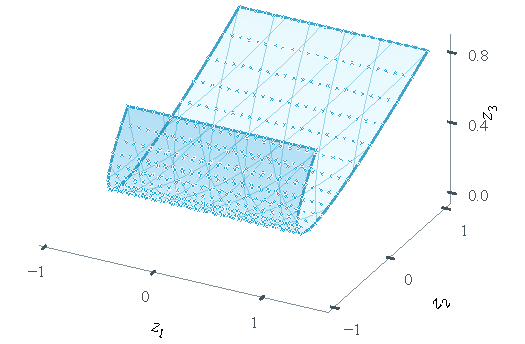
\includegraphics[width=\linewidth]{figures/io_trajectory/io_trajectory_paper.pdf}
 \caption{A curved family of complete input-output trajectories.
 Each point represents a length-two window
 $w=(u_0,u_1,y_0,y_1)^{\mathsf T}$ of $y_{k+1}=y_k^2+u_k$,
 selected with $u_1=-u_0$. The orthonormal coordinates
 $z=Q^{\mathsf T}w$ preserve the full vectors and their distances.
 The mesh follows the surface $z_3=\sqrt{2/3}\,z_2^2$;
 its curves do not represent evolution in time.}
 \label{fig:io-trajectory-example}
\end{wrapfigure}
Although the trajectory vectors belong to $\mathbb R^4$, the selected
family satisfies $u_0+u_1=0$ and is therefore contained in a
three-dimensional linear subspace. Let $Q$ have the orthonormal
columns $(1,-1,0,1)^{\mathsf T}/\sqrt3$,
$(0,0,1,0)^{\mathsf T}$, and
$(-1,1,0,2)^{\mathsf T}/\sqrt6$.
The coordinates $z=Q^{\mathsf T}w$ provide an exact visualization
of these complete trajectories: $w=Qz$, and
$\|w_i-w_j\|_2=\|z_i-z_j\|_2$.
Thus the three-dimensional picture retains both input samples
and both output samples through an invertible change of coordinates
on the selected subspace.

Substitution of~\eqref{eq:io-trajectory-example} gives
$z_1=\sqrt3a+x^2/\sqrt3$, $z_2=x$, and
$z_3=\sqrt{2/3}\,x^2$. As $(a,x)$ varies, the trajectory vectors
therefore trace a two-dimensional surface satisfying
$z_3=\sqrt{2/3}\,z_2^2$, as shown in
Fig.~\ref{fig:io-trajectory-example}. This parabolic cylinder
is curved despite having only two intrinsic dimensions; the
selected trajectories cannot all lie in a single two-dimensional
affine plane. The curvature reflects the nonlinear input-output
relation of the system and is preserved by the visualization.
The input restriction $u_1=-u_0$ is used only to obtain a
visualizable family of valid trajectories, rather than to
exhaust the system's finite-horizon behavior.
